\section{K-Nearest Neighbors}
In the same way as we have developed linear models, we have chosen to implement a model based on k nearest neighbors. We tuned the $k$ parameter to determine the optimal model. We also used the pipeline that was set up in the first examples to make the model as clear as possible and facilitate understanding.

\subsection{Model implementation}
\subsubsection{Implementation of a KNN model}
First, we set a simple knn model using the same pipeline we built in the last chapter. We then complexified the model to include cross-validation and parameter tuning to find the best hyper-parameters for our regression problem. We chose to \textbf{normalize} all the columns because of the properties of knn model (distance in space of features).

\subsubsection{Hyperparameters tuning}
As we did for the linear models, we chose to use \code{GridSearchCV} to tune the hyperparameter $k$ and find the fest model. By default (\href{https://scikit-learn.org/stable/modules/generated/sklearn.neighbors.KNeighborsClassifier.html}{scikit-learn documentation}), the model uses \textit{Minkowski} distance, but we chose to include distance function and how to weight neighbors' value.
\begin{lstlisting}
kf = KFold(n_splits=20, shuffle=True, random_state=42)
parameter = {
    'regressor__n_neighbors': np.arange(2, 30, 1),
    'regressor__metric': ['minkowski', 'euclidean', 'manhattan'],
    'regressor__weights': ['uniform', 'distance']
    }
...
knn_cv = GridSearchCV(knn, param_grid=parameter, cv=kf, verbose=1)
\end{lstlisting}
Then, we can extract the best hyperparameters from \code{regressor__n_neighbors} variable to train the tuned model.
\subsubsection{Check overfitting}
Learning curve (Figure~\ref{knn:learning-curve}) is a plot of the training and cross-validation error as a function of the training set size. It is a tool to find out how much we benefit from adding more training data and whether the estimator suffers more from a variance error or a bias error. We can use this to detect overfitting in the sense that a high training error and a low cross-validation error is a sign of overfitting.

\begin{figure}
    \centering
        \begin{subfigure}[b]{0.3\textwidth}
            \centering
            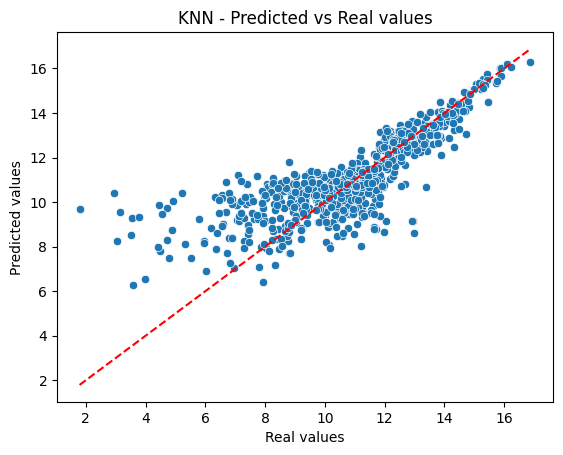
\includegraphics[width=\textwidth]{assets/images/knn-ypred-vs-ytest.png}
            \caption{$\hat{y}$ vs $y$ (log scale)}
            \label{knn:ypred-vs-yreal}
        \end{subfigure}
    \hfill
        \begin{subfigure}[b]{0.3\textwidth}
            \centering
            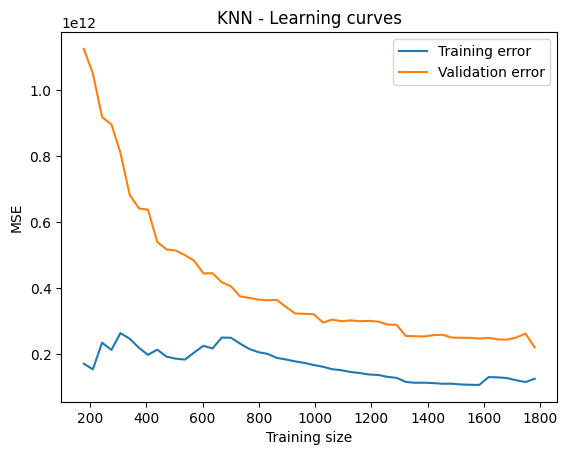
\includegraphics[width=\textwidth]{assets/images/knn-learning-curve.png}
            \caption{KNN learning curve}
            \label{knn:learning-curve}
        \end{subfigure}
    \hfill
        \begin{subfigure}[b]{0.3\textwidth}
            \centering
            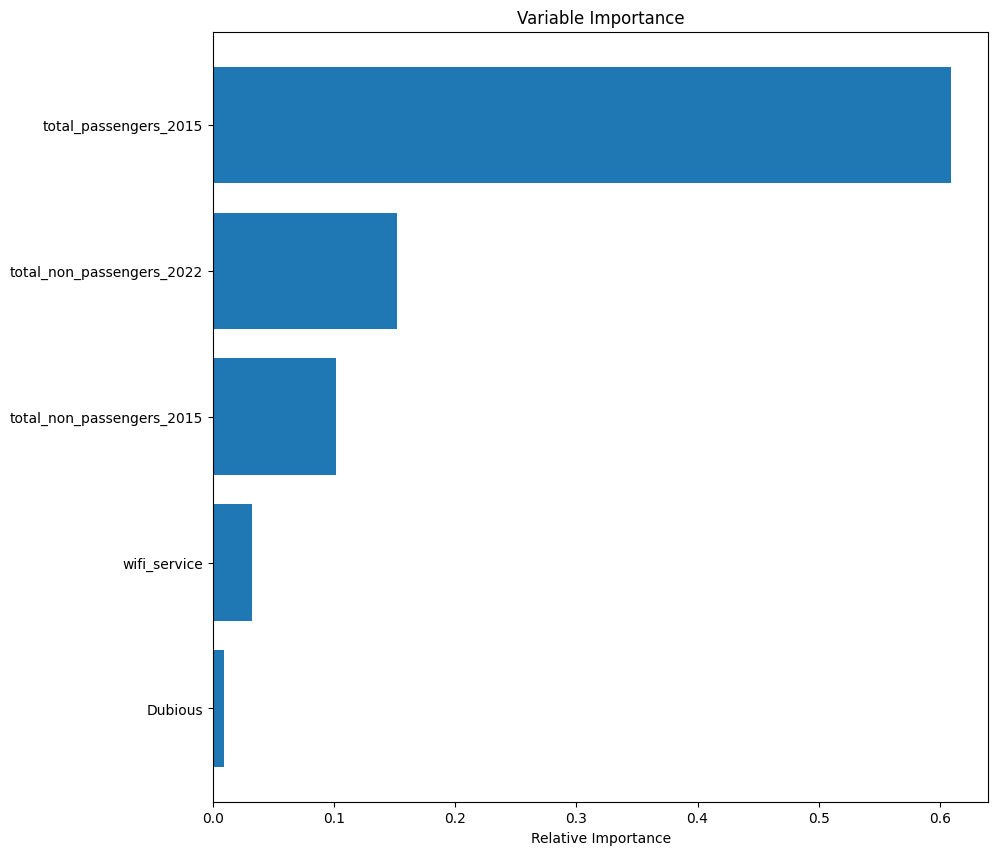
\includegraphics[width=\textwidth]{assets/images/knn-feature-importance.png}
            \caption{Feature importance}
            \label{knn:feature-importance}
        \end{subfigure}
    \caption{KNN metrics and performance analysis}
\end{figure}


\subsection{Results}
\subsubsection{Feature importance}
As the Lasso regularization, KNN models (tuned or raw) seems using quasi-only parameters related to train station (and not living area metrics) (see figure~\ref{knn:feature-importance}). As a consequence, we can ask if it it a good point to keep those very important features in the model. We conclude that, as the data is available, we should use it, like it would be in real problem solving.

\subsubsection{Performances}
Even if in linear scale, the KNN model seems to have good predictions, we can analyse $\hat{y}=f(y)$ (see figure \ref{knn:ypred-vs-yreal}). Indeed, we see that the model overestimates the traffic in train stations for low-traffic ones. This model is consequently adapted to our problem. Indeed, it is better to overestimate the traffic than just be flowed by too unpredicted people.

\begin{table}[h]
    \centering
    \begin{tabular}{ccccc}
        \toprule
        Model &  MSE &  MAE & MedianAE & $R^2$ Score \\
        \midrule
        Simple KNN model & 2.718e+11 & 140778 & 33152 & 0.834915\\
        KNN (best) & 2.176e+11 & 132651 & 30205 & 0.867865\\
        \bottomrule
    \end{tabular}
    \caption{Main metrics of KNN model}
\end{table}
We also see that the parameter tuning is useful, because we have $3,2$ points more for $R^2$ score (for instance).

\textbf{Observation:} As we don't have a lot of values for the high-traffic stations, the number of neighbors influence a lot the final prediction for those stations. Indeed, the points are really spread out, but knn model just compute the average of nearest points. This can lead to an unwanted approximation.